\documentclass[tikz,crop]{standalone}

\usepackage{tikz,pgfplots}
\usepackage{physics}

\usetikzlibrary{decorations.shapes}
\usetikzlibrary{arrows.meta,calc,decorations.markings,math,arrows.meta}
\usetikzlibrary{%
    decorations.pathreplacing,%
    decorations.pathmorphing%
}


%------------   Todo está en 2D porque no entiendo 3D   :c    ------------%


\begin{document}


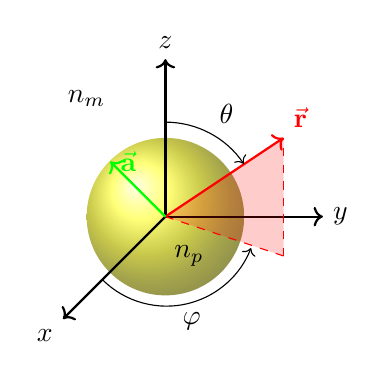
\begin{tikzpicture}[scale=1]
\shade[ball color=yellow, opacity = .7] (0,0) circle (1); 
\coordinate (O) at (0,0);



%draw the main coordinate system axes
\draw[thick,->] (O) -- (-1.3,-1.3) node[anchor=north east]{$x$};
\draw[thick,->] (O) -- (2,0) node[anchor= west]{$y$};
\draw[thick,->] (O) -- (0,2) node[anchor=south]{$z$};

\draw[thick,red,->] (O) -- (1.5,1) node[anchor=south west]{$\va{r}$};  %r=1.8, \theta=33.6
\draw[-, dashed,red] (O) -- (1.5,-.5);
\draw[-,dashed,red] (1.5,-.5) -- (1.5,1) ;

\fill[red,opacity=.2] (O)--(1.5,-.5)--(1.5,1)--(O);
	
\path (O)++(62:1.2)node[anchor=south west]{$\theta$};    
\draw[->](0,1.2)arc(90:34:1.2);

\path (O)++(-85:1.1)node[anchor=north west]{$\varphi$};    
\draw[->](-.8,-.8)arc(-135:-21:1.15);
	
	
\draw[thick,green,->] (O) -- (-.7,.7) node[anchor=west]{$\va{a}$};  

\path (O)++(.3,-.5) node{$n_p$};
\path (O)++(-1,1.5) node{$n_m$};

	
\end{tikzpicture}

\end{document}